\providecommand{\main}{../../../..}
\documentclass[\main/dresen_thesis.tex]{subfiles}

\begin{document}
  \begin{figure}[tb]
    \centering
    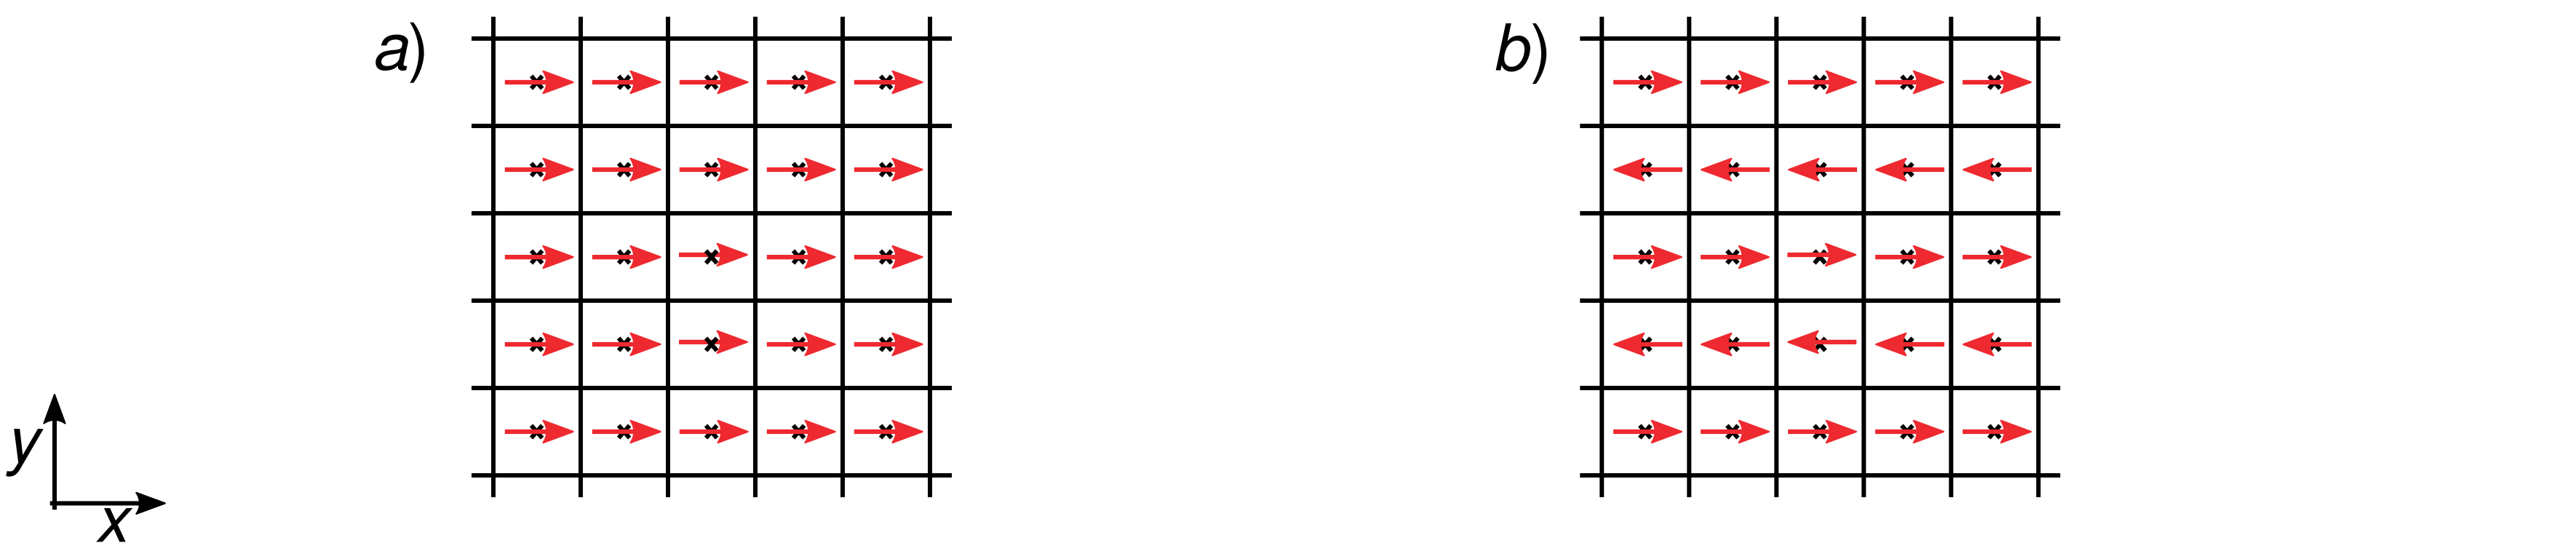
\includegraphics{monolayers_theo_sum}
    \caption{\label{fig:monolayers:magnetism:theoSum}Depiction of two considered magnetic configurations on a square lattice: (a) super ferromagnetic and (b) super antiferromagnetic.}
  \end{figure}


  The energy gain only due to dipolar interaction for a transition of a square array from a perfectly aligned super ferromagnetic state towards a super antiferromagnetic state is calculated for zero temperature by performing a double sum over all lattice sites from the point of view of a single magnetic moment.
  Consider the magnetic moment situated in a plane at the origin $(0, \,0)$ with its moment aligned to the $y$ axis $\mu_{00} \eq \mu \hat{e}_y$, and the other magnetic moments at the coordinates $(i a_{pp}, j a_{pp})$, where $i,\, j$ are integer numbers and $a_{pp}$ is the spacing between two particles on the square lattice.
  In the super ferromagnetic case all magnetic moments are considered to point along the $y$ direction $\mu_{ij} \eq \mu \hat{e}_y$, whereas for the super antiferromagnetic case the direction is alternating with the $x$-coordinate $\mu_{ij} \eq (-1)^i \mu \hat{e}_y$.
  The two lattices are depicted in \reffig{fig:monolayers:magnetism:theoSum}.
  % figure einfügen.
  The energy is then determined by calculating the Zeeman energy of $\mu_{00}$ with the dipolar magnetic field described in \refeq{eq:theoreticalBackground:magnetism:dipolarField} generated by all the other moments $\mu_{ij}$, which reads
  \begin{align}
    E \eq -\sideset{}{'}\sum_{i,j=-\infty}^\infty \frac{\mu_0}{4 \pi} \frac{3(\vec{\mu_{ij}} \cdot \hat{r})(\vec{\mu_{00}} \cdot \hat{r}) - \vec{\mu_{ij}} \cdot \vec{\mu_{00}} }{r^3},
  \end{align}
  where $r \eq \sqrt{i^2 + j^2} a_{pp}$.
  The explicit sum for super ferromagnetic and super antiferromagnetic states is then given by
  \begin{align}
    E^\mathrm{SFM} \eq -\frac{\mu_0 \mu^2}{4 \pi a^3_{pp}} \sideset{}{'}\sum_{i,j=-\infty}^\infty  \frac{3j^2}{(i^2 + j^2)^{5/2}} - \frac{1}{(i^2 + j^2)^{3/2}} ,\\
    E^\mathrm{SAFM} \eq -\frac{\mu_0 \mu^2}{4 \pi a^3_{pp}} \sideset{}{'}\sum_{i,j=-\infty}^\infty (-1)^i \biggl( \frac{3j^2}{(i^2 + j^2)^{5/2}} - \frac{1}{(i^2 + j^2)^{3/2}} \biggr).
  \end{align}
  Numerically, both sums can be solved up to the desired precision, which yields a practical expression for the energy gain per particle on an infinite lattice
  \begin{align}
    E^\mathrm{SFM} &\eq -4.52 \frac{\mu_0 \mu^2}{4 \pi a^3_{pp}},\\
    E^\mathrm{SAFM} &\eq -5.10 \frac{\mu_0 \mu^2}{4 \pi a^3_{pp}},\\
    \Delta E &\eq -0.58 \frac{\mu_0 \mu^2}{4 \pi a^3_{pp}}.
  \end{align}

  For the studied square lattices in this chapter, which both have particles with magnetic moments in the order of $\mu \eq 23000 \mu_B$ and square lattices with spacing in the order of $13 \unit{nm}$, the energy gain corresponds to $7.5 \unit{meV}$, which corresponds to $87 \unit{K}$ or an effective magnetic field of $\Delta E / \mu \eq 6 \unit{mT}$ for the nanocubes.
  As this is a relatively low energy scale, it is expected that low temperatures and low magnetic field are necessary to observe an undisturbed super antiferromagnetic state.
\end{document}